\documentclass{article}

\title{Prova Finale di Reti Logiche\\ \large Politecnico di Milano}
\author{Lorenzo Gadolini, \\ Giuseppe Lischio}
\usepackage[a4paper, includeheadfoot,margin=2cm]{geometry}
\usepackage{amsfonts}
\usepackage{amsmath}
\usepackage{graphicx}
\graphicspath{{./Images/}}
\usepackage{mathrsfs}
\usepackage{siunitx}
\usepackage{systeme}
\usepackage{textcomp}
\usepackage{xcolor}
\usepackage{wrapfig}
\usepackage{tikz}
\usepackage{MnSymbol}
\usepackage{tocbibind}
\usepackage[toc,page]{appendix}

\newenvironment{codeFont}{\fontfamily{pcr}\selectfont}{\par}
\newenvironment{gitFont}{\fontfamily{zi4}\selectfont}{\par}



\begin{document}

\maketitle

\pagenumbering{Roman}

\tableofcontents


\newpage
\pagenumbering{arabic}




\setcounter{page}{1}


\section{Introduzione}
\begin{flushleft}
Il metodo di codifica a working-zone propone un'ottimizzazione orientata alla riduzione del consumo di energia introdotto dall'input/output di un microprocessore.

\medskip

Sia dato un generico sistema composto da un processore e una memoria esterna al chip referenziabile tramite un bus indirizzi. Questo metodo suggerisce che un programma in esecuzione sul dato sistema sfrutti durante la sua esecuzione un insieme di indirizzi "preferiti", e che quindi sia più efficiente racchiudere tutti questi indirizzi dentro uno spazio di lavoro (detto appunto Working-Zones). 

\medskip

Gli indirizzi di queste Working-Zones sono codificati tramite un sistema base e offset, così da ridurre ulteriormente la quantità di informazione trasmessa sul bus indirizzi, e di conseguenza ridurre anche l'energia dissipata.

\end{flushleft}
\subsection{Dati Progettuali e Specifica}
\begin{flushleft}

Il componente da progettare ha come compito quello di stabilire se un indirizzo che riceve in input appartiene o meno ad una delle Working-Zones stabilite, e in caso affermativo di effettuare la traduzione dell'indirizzo da binario naturale a codifica WZE.

\medskip

Il componente si interfaccia con una memoria indirizzabile al byte a partire dall'indirizzo 0, e in cui vengono inizializzati i dati necessari per effettuare la computazione. La memoria inoltre è indirizzabile tramite indirizzi di 16 bit.

\medskip

Gli indirizzi di memoria da 0 a 7 contengono le basi delle 8 Working-Zones stabilite in fase di setup e scritte in binario naturale senza segno su 7 bit.
\smallskip

La cella di memoria 8 contiene l'indirizzo su cui effettuare la verifica e l'eventuale codifica, anch'esso scritto in binario naturale senza segno su 7 bit.
\smallskip

L'indirizzo di memoria 9 conterrà a fine computazione un numero di 8 bit senza segno, che come verrà descritto più avanti potrà essere una codifica o un indirizzo semplice.

\medskip

I restanti indirizzi sono tutti inizializzati a 0 e non vengono sfruttati durante la computazione.

\end{flushleft}
\subsection{La fase di traduzione}
\begin{flushleft}

Nella fase di codifica il componente deve essere in grado di stabilire se un indirizzo depositato nella cella numero 8 della memoria appartiene o meno ad una Working-Zone.

\medskip

Un indirizzo che non appartiene a nessuna Working-Zone fa entrare il componente in uno stato di "Non appartenenza", stato in cui la macchina secondo specifica deve depositare in uscita il dato così come le è stato fornito, preceduto da un bit posto a "0".
\smallskip

Il dato in uscita è un intero binario naturale senza segno di 8 bit

\bigskip

\begin{gitFont}

"0" \& "0101010"  \ \  --Codifica\footnote{Il simbolo \& indica concatenazione di bit} esempio di indirizzo che non cade in alcuna WZ

\end{gitFont}

\bigskip

Se il componente stabilisce che l'indirizzo appartiene ad una Working-Zone, scatta la fase di "Appartenenza", il dato necessita di encoding.
\smallskip

Un indirizzo codificato è un numero di 8 bit senza segno composto da tre sottogruppi di bit.

\begin{itemize}
\item Il bit più significativo viene posto ad "1", che indica "Codifica avvenuta";
\item I tre bit successivi codificano posizionalmente la Working-Zone a cui tale indirizzo appartiene. Il dato in uscita è un numero binario naturale senza segno da 0 a 7 che indica che l'indirizzo appartiene alla "n-esima" Working-Zone.

\newpage

\item I quattro bit finali codificano l'offset dell'indirizzo dalla base. Il numero codificato è un numero binario One Hot. L'offset indica la distanza posizionale in memoria dall'indirizzo base, ovvero l'indirizzo "si trova a" n indirizzi dalla base.  %%Se si crea un appendice, spiegare la codifica one hot.
\end{itemize}

\bigskip


\begin{gitFont}

"1" \& " 010" \& " 0100"  \ \ --Codifica esempio di indirizzo appartenente ad una WZ

\end{gitFont}


\bigskip

Sia che l'indirizzo appartenga o che non appartenga ad una Working-Zone, il componente prosegue sempre lungo la stessa fase di output. Il dato viene depositato in memoria, salvato, e la macchina entra in fase di attesa di reset e avvio per una successiva codifica.
\end{flushleft}
\subsubsection{Entity del componente}

Il componente hardware è stato progettato tramite linguaggio VHDL in base alle specifiche fornite dal tema di progetto.

La struttura input/output del componente in VHDL è stata fornita nelle specifiche ed è di seguito riportata.


\begin{center}
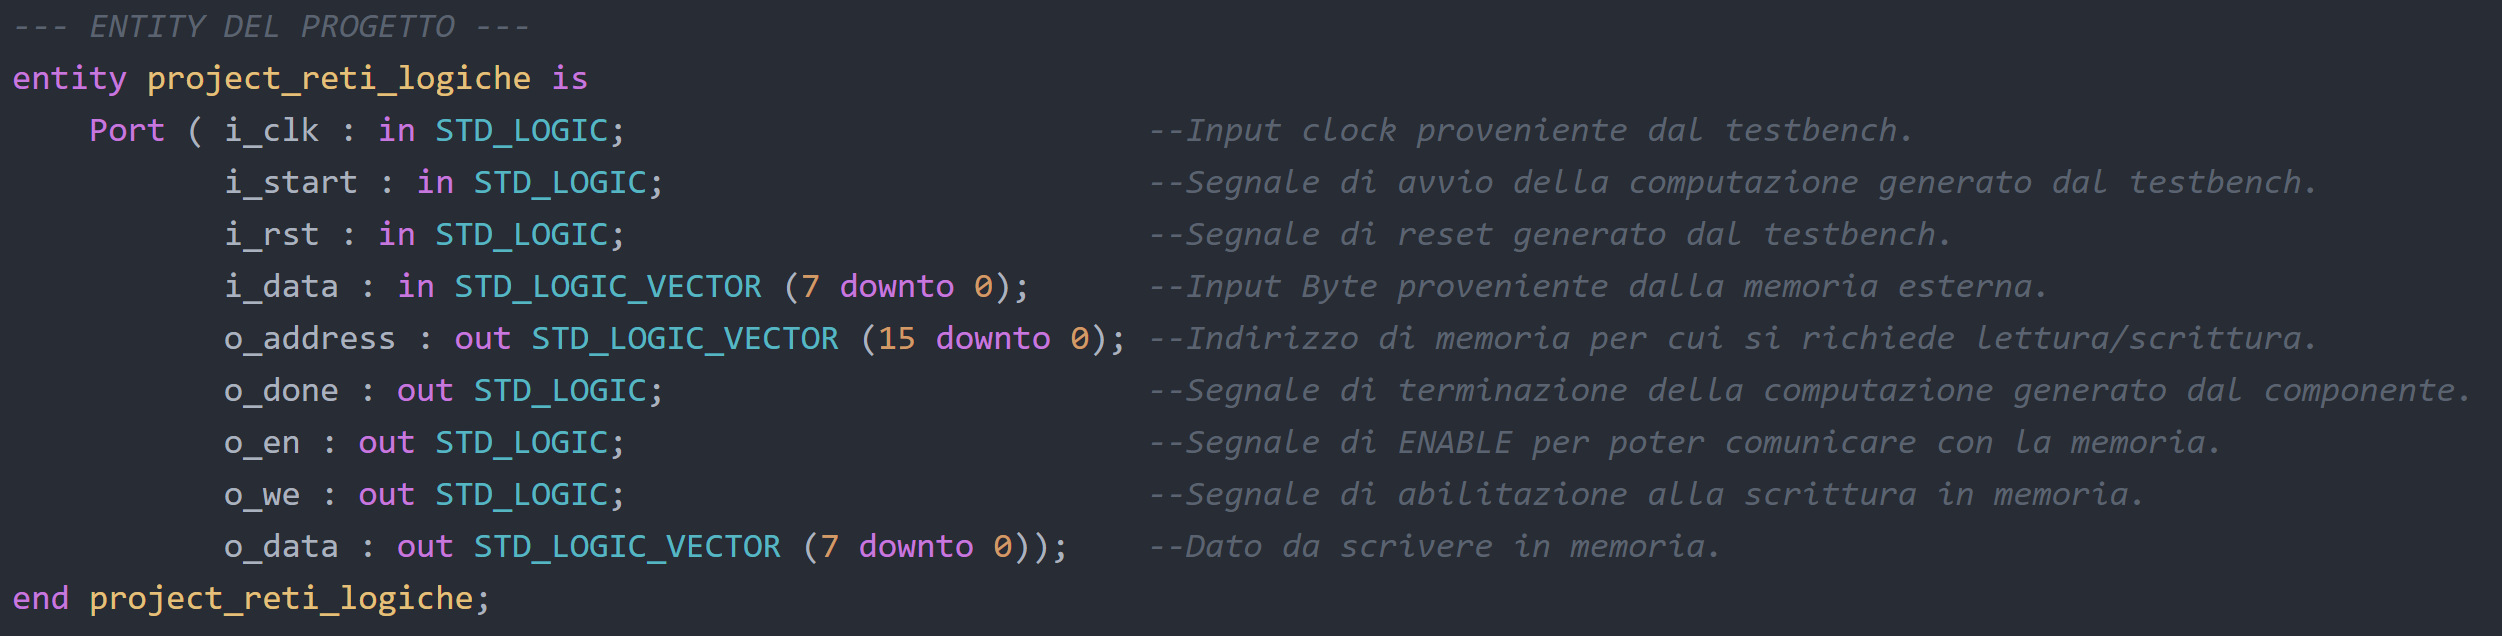
\includegraphics[scale=0.27]{Entity}
\end{center}


\section{Architettura e Scelte Progettuali}

\subsection{L'algoritmo}

\begin{flushleft}


Il progetto si basa su un algoritmo alquanto semplice.
\smallskip

Dato uno stato iniziale di memoria, per prima cosa viene letto il dato di cui si necessita la codifica dall'indirizzo di memoria numero 8, successivamente il componente entra in un ciclo di calcolo. In questo ciclo di calcolo vengono letti uno alla volta i byte di memoria 0-7 contenenti gli indirizzi base delle Working zones.
\smallskip

 Il componente sottrae l'indirizzo da codificare all'indirizzo base letto, e verifica che il risultato cada fra 0 e 3. Questo risultato ha il significato di offset, e come da specifica, un offset compreso fra 0 e 3 (inclusi) indica un'appartenenza alla working zone. Qualsiasi altro risultato viene interpretato come "Non appartenenza".

\subsection{Non Appartenenza}\label{notA}

Un risultato che non appartiene a nessuna working zone deve venire propagato in uscita così come è stato letto da memoria in entrata. Il componente ha terminato gli otto cicli di verifica e ha determinato che l'indirizzo in input non appartiene a nessuna working zone. A questo punto la macchina carica i 7 bit dell'indirizzo nel registro di output, il quale era stato inizializzato con 8 bit tutti posti a zero, così da rispettare la specifica che prevede di emettere in uscita uno 0 seguito dai 7 bit dell'indirizzo scritti in binario naturale senza segno.

\newpage

\subsection{Appartenenza}\label{app}

Se il componente durante la sua esecuzione verifica che l'indirizzo da codificare cade all'interno di una delle basi, allora si avvia la procedura di encoding. Per prima cosa viene codificato l'offset. Il risultato della sottrazione appartiene ad un insieme finito e ristretto di valori, per questo si è scelto di creare una lookup table che contenesse le codifiche in onehot da assegnare al valore di uscita a seconda del valore di offset.
Una volta scritto in memoria il primo quartetto di bit, il componente passa alla traduzione della tripletta di bit contenente l'indirizzo della working zone. Questa fase scrive i tre bit nel registro di out che corrispondono al valore binario naturale del byte di memoria che contiene l'indirizzo base.

Infine il componente pone ad 1 il MSB del valore di uscita, cosi che chi riceve il valore tradotto a valle riconosce che è stato effettuato l'encoding.


\end{flushleft}
\subsection{Il design: La macchina a stati}

Il progetto del componente parte dalla descrizione di una macchina a stati che esegua l'algoritmo poco fa descritto

La macchina a stati completa che esegue la codifica è disegnata qui:

\begin{flushleft}
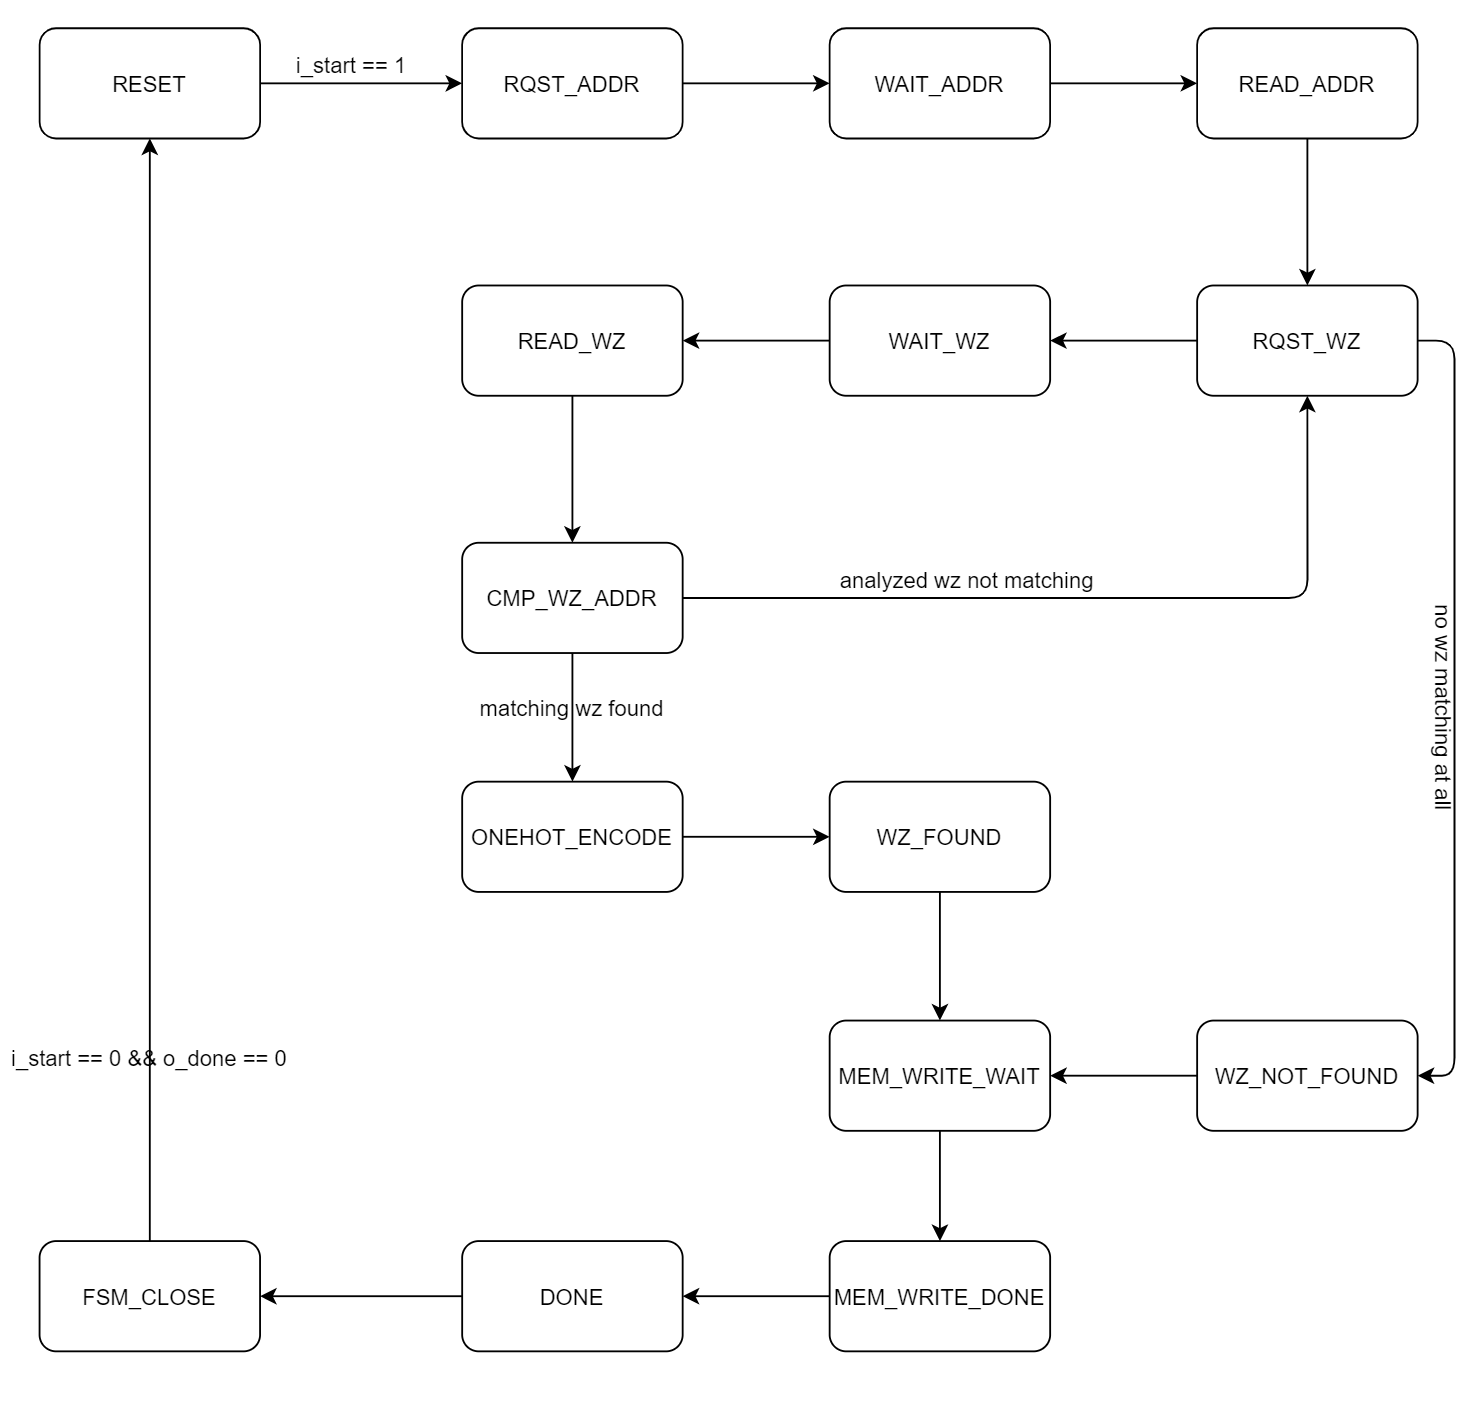
\includegraphics[scale=0.40]{FSM}
\end{flushleft}

Nel paragrafo \ref{fsm} verranno descritti i compiti dei singoli stati e delle transizioni.

\newpage

\subsubsection{Descrizione degli stati}\label{fsm}

\begin{itemize}

\item RESET: Lo stato in cui la macchina viene avviata e a cui giunge una volta che riceve il segnale di reset. La macchina cicla su questo stato attendendo un segnale di start. Successivamente inizializza la memoria e salta al primo vero stato di esecuzione.

\item RQST\_ ADDR: La macchina richiede alla memoria l'indirizzo da codificare.

\item WAIT\_ ADDR: La macchina attende per un ciclo di clock la propagazione dei segnali alla memoria.

\item READ\_ ADDR: La macchina ottiene il dato dalla memoria.

\item RQST\_ WZ: La macchina richiede alla memoria il valore della n\_ esima base, dove n è compreso fra 0 e 7.

\item WAIT\_ WZ: La macchina attende un ciclo di clock la propagazione dei segnali alla memoria.

\item READ\_ WZ: La macchina ottiene la base n-esima dalla memoria.

\item CMP\_ WZ\_ ADDR: La macchina esegue la sottrazione che determina l'appartenenza o meno e l'offset del dato da codificare.

\item ONEHOT\_ ENCODE: La macchina codifica l'offset di un indirizzo che ha dato esito positivo in una comparazione.

\item WZ\_ FOUND: La macchina prepara il byte contenente il dato codificato e notifica alla memoria che è pronto per essere scritto

\item WZ\_ NOT\_ FOUND: La macchina notifica alla memoria che il dato non appartiene a nessuna Working Zone, e che è pronta a propagarlo senza codifica.

\item MEM\_ WRITE \_ WAIT: La macchina attende un clock che la memoria riceva la sua richiesta di scrittura

\item MEM\_ WRITE\_ DONE: La macchina completa la fase di scrittura.

\item DONE: La macchina notifica il raggiungimento dello stato di terminazione.

\item FSM\_ CLOSE: La macchina entra in attesa di una richiesta di reset.

\end{itemize}

\begin{flushleft}


Nel grafico della macchina è stato escluso l'autoanello dello stato di reset. L'autoanello è necessario perchè permette alla macchina di rimanere in attesa su tale stato che il segnale di start si alzi, dando il via ad una nuova computazione.
\smallskip

 Sono stati inoltre esclusi tutti gli archi che da ogni singolo stato portano allo stato di reset.
\begin{gitFont}i{\_}rst \end{gitFont} potrebbe venire posto alto (ad "1") in qualsiasi momento della computazione. 
\smallskip

Data questa evenienza è necessario che la macchina in qualsiasi stato si trovi abbandoni l'encoding ed entri nello stato di reset. 
\smallskip

Questo si ottiene con una gestione asincrona della verifica del segnale. 
Ad ogni ciclo di clock viene analizzato il segnale, e se posto ad "1" la macchina esegue una transizione allo stato in cui si trova a RESET.


\end{flushleft}

\subsection{Il Codice VHDL}

\begin{flushleft}


Fino a questo momento non è stata data nessuna descrizione fisica del componente al di fuori delle specifiche che descrivono il problema. In questo piccolo paragrafo viene fatta un'analisi di come è stata descritta la macchina a stati in linguaggio VHDL, analizzandone i segnali e i registri necessari al funzionamento.

Il componente è stato descritto tramite codice VHDL Behavioral che implementa tutti gli stati descritti nel paragrafo \ref{fsm}.

 Oltre all'architettura fornita dalla specifica, il componente possiede altri segnali e registri che si sono resi necessari in fase di scrittura di codice.

\begin{flushleft}
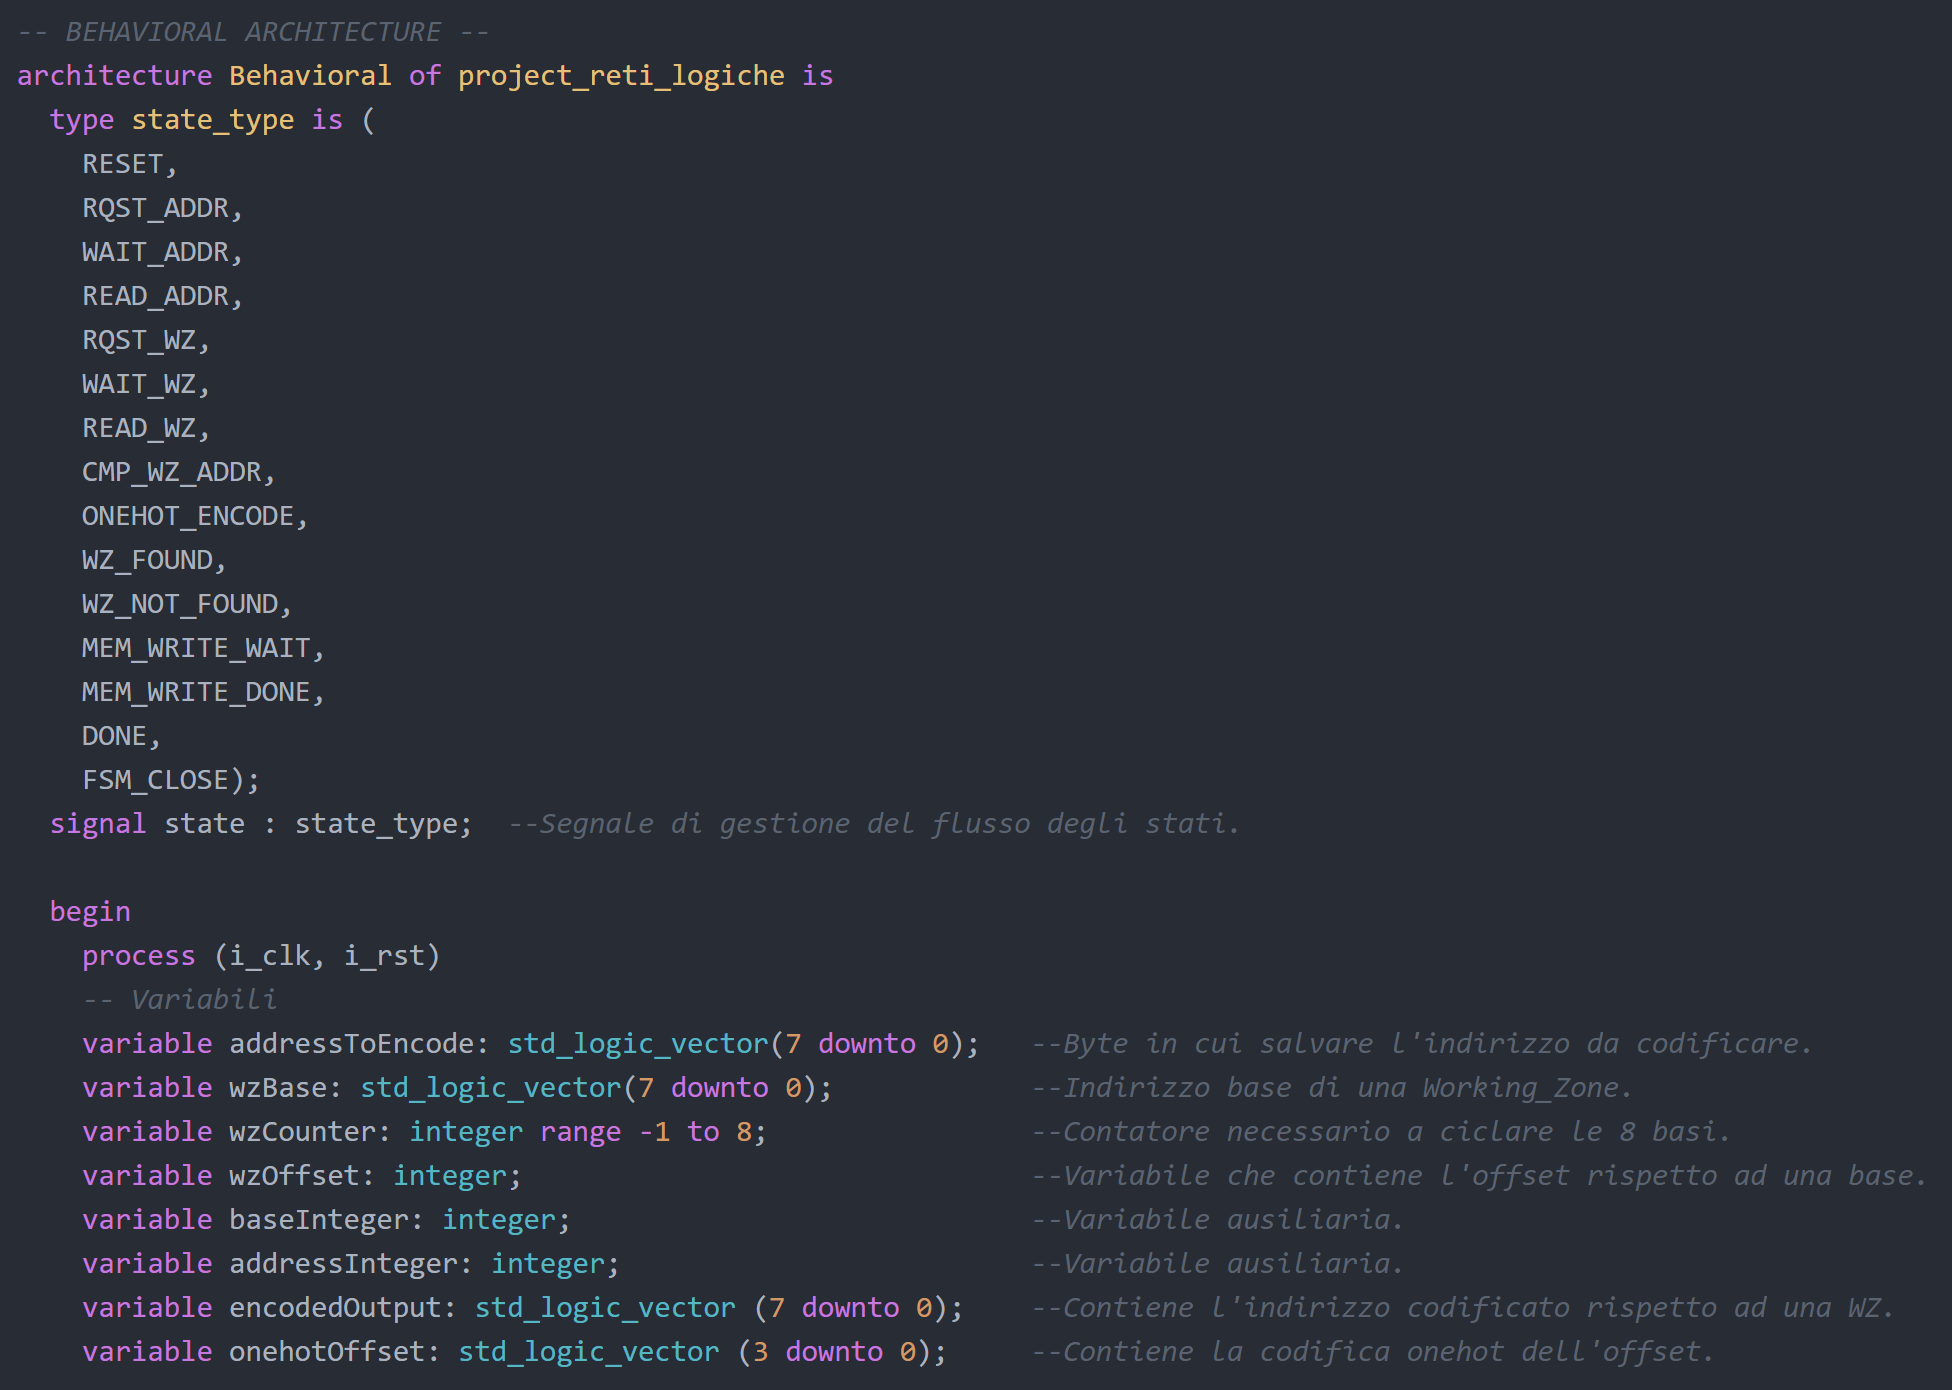
\includegraphics[scale=0.31]{Behavioral}
\end{flushleft}


\begin{itemize}

\item \begin{gitFont}
addressToEncode
\end{gitFont} Variabile di tipo std{\_}logic{\_}vector a 8 bit, viene utilizzata per salvare l'indirizzo che necessita di valutazione e codifica.

\item \begin{gitFont}
wzBase
\end{gitFont} Variabile std{\_}logic{\_}vector a 8 bit che salva nel ciclo di computazione la base della Working-Zone e viene aggiornata ad ogni risultato di non appartenenza con la base successiva.

\item \begin{gitFont}
wzCounter
\end{gitFont} Variabile integer che  può assumere valori da -1 (default) ad 8. Viene sfruttata come flag per segnalare a quale valore di byte in memoria siamo arrivati. Raggiunto il valore 8 funge da flag per segnalare al componente che non ci sono più Working-Zones da valutare e che la macchina deve entrare in stato di "Non Appartenenza" (par. \ref{notA}).

\item \begin{gitFont}
wzOffset
\end{gitFont} Variabile integer che salva il valore dell'offset di un indirizzo rispetto alla sua base in caso la macchina determini che tale indirizzo appartiene ad una Working-Zone.

\item \begin{gitFont}
encodedOutput
\end{gitFont} Variabile di tipo std{\_}logic{\_}vector a 8 bit che salva un indirizzo che è stato sottoposto a processo di encoding ( par. \ref{app}).

\item \begin{gitFont}
encodedOutput
\end{gitFont} Variabile di tipo std{\_}logic{\_}vector a 4 bit che viene sfruttata dalla macchina per salvare il valore di offset in codifica onehot.

\end{itemize}

\end{flushleft}
\section{Risultati della Sintesi}
Il componente progettato è stato sintetizzato in maniera virtuale tramite l'apposito tool di Vivado. La sintetizzazione ha dato un risultato positivo, ed il componente è stato successivamente testato anche post sintesi, con gli stessi test effettuati per il solo funzionamento logico. Inoltre è emerso che il componente funziona correttamente anche impostando periodi di clock molto inferiori al requisito minimo della specifica (100 ns). Qui di seguito il dettaglio dei segnali del componente durante un test con clock a 5 ns:

%%da aggiungere screen con il dettaglio dei segnali con clock tipo a 10ns


\section{Simulazioni}

In questo paragrafo verranno discussi i metodi utilizzati per verificare il corretto funzionamento del componente progettato. In particolare è stato usato il software Xilinx "Vivado" per scrivere i test bench e per effettuare vari tipi di simulazione:

\begin{itemize}

\item Simulazione \textbf{Behavioral}: test del funzionamento logico del componente, basato sul codice VHDL scritto, senza passare per la sintesi virtuale del componente.

\item Simulazione \textbf{Post-Synthesis Functional}: test che permette di verificare il comportamento strutturale del componente descritto. Viene eseguito dopo aver terminato il processo di sintesi virtuale

\item Simulazione \textbf{Post-Synthesis Timing}: test analogo al \textit{Post-Synthesis Functional}, che tiene però conto di tutti i ritardi introdotti dalle porte logiche usate nella simulazione del componente virtuale.

\end{itemize}



%%poi da fare un elenco con i vari test bench eseguiti, spiegando cosa si è andato a testare. In particolare per il testing post sintesi timing fare il discorso su i vari test fatti con il periodo di clock sempre più corto.

\section{Conclusioni}


\end{document}
